\normaltrue \difficilefalse \tdifficilefalse
\correctionfalse

%\UPSTIidClasse{11} % 11 sup, 12 spé
%\newcommand{\UPSTIidClasse}{12}

\exer{La Seine Musicale $\star$ \label{B2:14:39}}
\setcounter{question}{0}\UPSTIcompetence[2]{B2-14}
\index{Compétence B2-14}
\index{La Seine Musicale}
\ifcorrection
\else
\textbf{Pas de corrigé pour cet exercice.}
\fi

\ifprof
\else
On choisit de représenter une demi-voile, de repère $\rep{v}\repere{O}{x_v}{y_v}{z}$, par une portion de demi-sphère (\autoref{fig_39_01}).
On pourra remarquer qu’il n’y a pas de mouvement relatif entre les repères $\rep{C_G}\repere{C_G}{x_{C_G}}{y_{C_G}}{z}$ et $\rep{v}\repere{O}{x_v}{y_v}{z}$, 
associé à la demi-voile. On rappelle que $\vect{OC_G}=R\vect{y_{C_G}}$, avec $R$ le rayon moyen de la voie de roulement.


\begin{figure}[H]
\centering
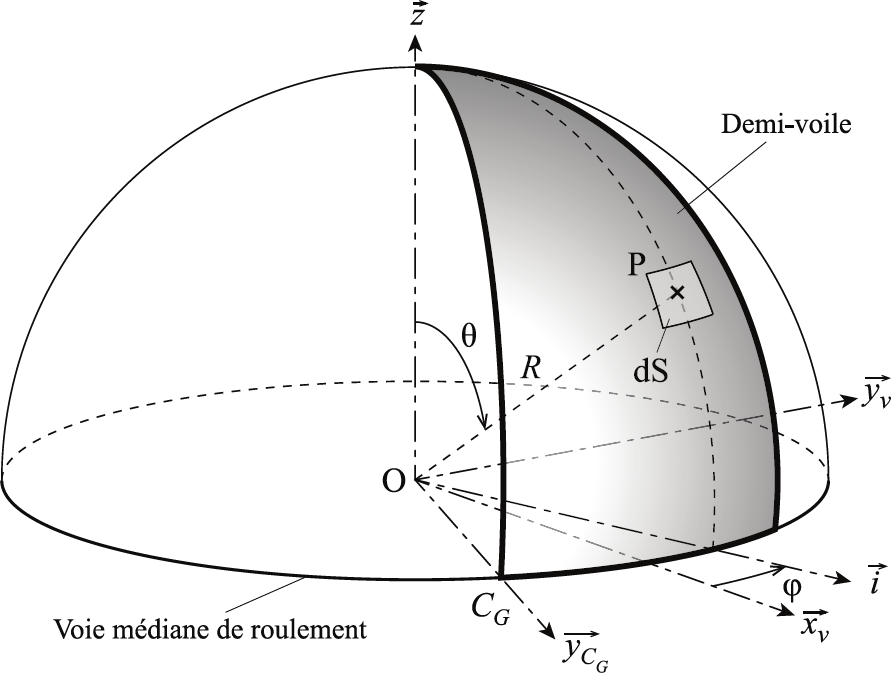
\includegraphics[width=\linewidth]{39_01}
\caption{Paramétrage de la surface totale et élémentaire en coordonnées sphériques de la demi-voile \label{fig_39_01}}
\end{figure}

La figure \autoref{fig_39_02} présente l’orientation du vent par rapport au plan de symétrie de la demi-voile dans le plan $\angl{x_v}{y_v}$. La densité d’effort surfacique du vent sur la demi-voile, pour une vitesse de $\SI{9}{m.s^{-1}}$, est noté $\vect{f}_{\text{vent}}=f\vect{u}$ avec $f=\SI{54,7}{N.m^{-2}}$, l’orientation de $\vect{u}$ étant définie par l’angle constant $\alpha=\angl{x_v}{u}$.

La base associée au système de coordonnées sphériques $\left(r,\theta,\varphi\right)$ est $\base{e_r}{e_{\theta}}{e_{\varphi}}$. La position du point $P$ appartenant
à la demi-voile est définie par $\vect{OP}=R\vect{e_r}$ avec $R$ le rayon moyen de la voie de roulement ($R=\SI{22,75}{m}$).
L’angle azimutal $\varphi$ évolue entre $-\dfrac{\pi}{8}$ et $\dfrac{\pi}{8}$ et l’élévation $\theta$ évolue entre 0 et $\dfrac{\pi}{2}$.
On précise que, dans le cas présenté \autoref{fig_39_01}, la surface élémentaire en coordonnées sphériques est notée
$\dd S =R^2 \sin \theta \dd\theta \dd \varphi$.


\begin{figure}[H]
\centering
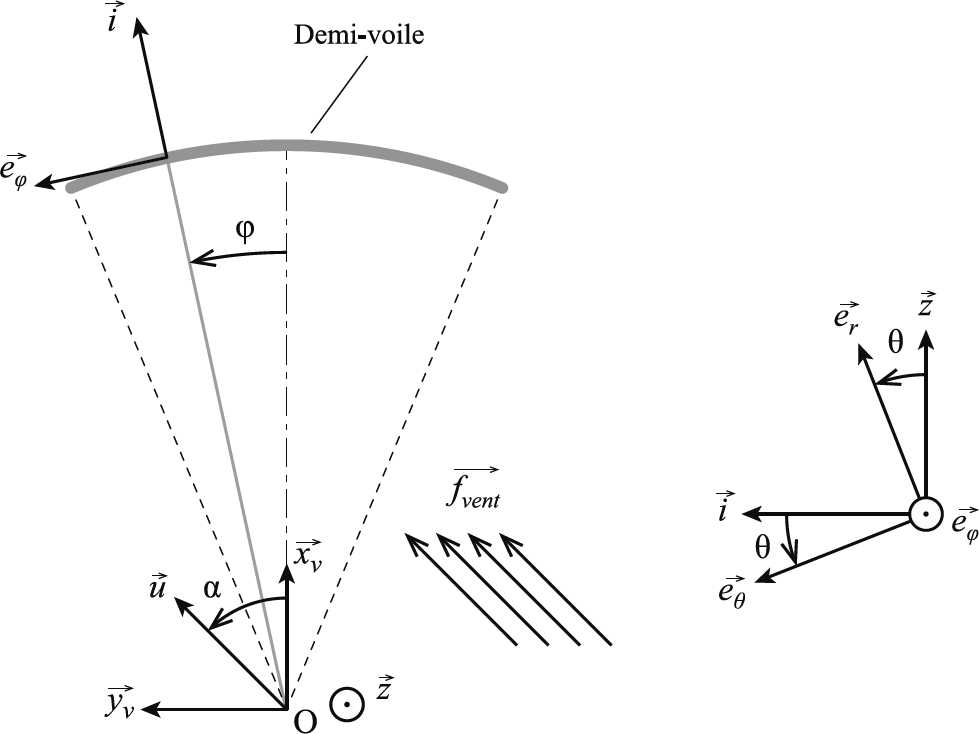
\includegraphics[width=\linewidth]{39_02}
\caption{Paramétrage angulaire \label{fig_39_02}}
\end{figure}

\fi




\question{Exprimer l’effort élémentaire du vent sur la demi-voile s’appliquant au point $P$ sur la surface $\dd S$, noté $\dd \vect{F}_{\text{vent}}$.}
\ifprof
\else
\fi

\question{Déterminer par intégration l’expression du moment de l’action mécanique du vent selon l’axe $\axe{O}{z}$, $\vectm{O}{\text{vent}}{\text{demi-voile}} \cdot \vect{z}$ s’opposant à la rotation de la voile autour de l’axe $\axe{O}{z}$ en fonction de $R$, $f$ et $\alpha$.}
\ifprof ~\\
\else
\fi

\question{On définit ${F}_{\text{vent}}$ tel que 
$\left(\vect{OC_G}\wedge {F}_{\text{vent}} \vect{x_{C_G}}\right)\cdot \vect{z} = \vectm{O}{\text{vent}}{\text{demi-voile}} \cdot \vect{z}$. 
En déduire l’expression de ${F}_{\text{vent}}$ l’effort
du vent au point $C_G$ s’opposant au déplacement du chariot central.}
\ifprof ~\\
\else
~\\
Afin de modéliser le déplacement de la voile dans le cas le plus défavorable, on souhaite déterminer la valeur
maximale de $\left| {F}_{\text{vent}}\right| $.
\fi

\question{Pour quelle valeur de $\alpha$ cet effort est-il maximal ? Déterminer la valeur maximale de $\left| {F}_{\text{vent}}\right| $.}
\ifprof ~\\
\else
\fi


\ifprof
\else
\begin{flushright}
\footnotesize{Corrigé  voir \ref{B2:14:39}.}
\end{flushright}%
\fi